% ----------------------------------------------------------
% Capítulo 2 -- Contexto do Projeto
% ----------------------------------------------------------
\chapter{Contexto do Projeto}\label{cap:contexto}

Este capítulo apresenta o contexto atual no qual o projeto \textit{SyncCarreira} está inserido, caracterizando o cenário histórico e mercadológico da orientação vocacional, o público diretamente envolvido, as necessidades identificadas a partir desse cenário e as regras de negócio do domínio. O objetivo é estabelecer a compreensão do problema sob a perspectiva da comunidade atendida (instituições, profissionais de orientação e jovens), ainda de forma independente da solução computacional, que será detalhada nos capítulos seguintes.

\section{Cenário}\label{sec:cenario}

A trajetória da Orientação Profissional (OP) no Brasil é marcada por transformações teóricas e metodológicas que acompanham as mudanças políticas, sociais e econômicas do país \cite{abade2005}. As primeiras aplicações sistemáticas da Psicologia ao trabalho ocorreram na década de 1920, voltadas à seleção profissional em cursos técnicos e empresas ferroviárias, sob a lógica do ``homem certo no lugar certo'' \cite{abade2005}. Esse período psicométrico consolidou-se com a criação do Instituto de Seleção e Orientação Profissional (ISOP), em 1947, que utilizava testes vocacionais para direcionar indivíduos de acordo com aptidões inatas, frequentemente desconsiderando condições de classe e histórias de vida \cite{abade2005}.

A partir da década de 1960, essa hegemonia psicométrica começou a ser questionada. Sob influência da abordagem clínica proposta pelo psicólogo argentino Rodolfo Bohoslavsky, a orientação profissional passou a compreender a escolha de carreira não como o ajuste de um perfil fixo a uma profissão, mas como um processo de esclarecimento em que o indivíduo é auxiliado a assumir sua própria capacidade de decidir \cite{bohoslavsky2015}. No Brasil, essa perspectiva clínica foi introduzida e adaptada por Maria Margarida Moreira Jorge de Carvalho, da Universidade de São Paulo, cuja tese de doutorado sistematizou a orientação profissional em dinâmica de grupo --- metodologia que passou a integrar a aprendizagem experiencial e cognitiva do estudante ao processo de escolha, e que deu origem ao Serviço de Orientação Profissional do Instituto de Psicologia da USP \cite{carvalho1979}.

Nas décadas seguintes, a área passou a incorporar críticas às abordagens que ignoravam desigualdades sociais e atribuíam ao indivíduo isolado a responsabilidade por seu sucesso ou fracasso profissional. A escolha de carreira consolidou-se, então, como um processo multideterminado e dinâmico \cite{abade2005}, compreendido a partir de uma perspectiva sócio-histórica como uma construção social --- e não como a revelação de uma vocação inata e imutável \cite{bock2004}. Essa mudança de paradigma permanece como a base conceitual predominante na literatura contemporânea: revisão de escopo sobre intervenções em Orientação Profissional fundamentadas nas abordagens histórico-cultural e sócio-histórica, que mapeou a produção científica nacional entre 2013 e 2023, confirma essa predominância teórica e evidencia que tais intervenções ocorrem majoritariamente em grupo, com adolescentes e jovens, no contexto escolar ou em organizações sociais voltadas à inserção do jovem no mercado de trabalho \cite{martins2024}. A mesma revisão constata que, embora a Lei nº 13.935/2019 tenha tornado obrigatória a presença de psicólogos na rede pública de educação básica, essa presença ainda não se consolidou na maioria das escolas brasileiras, o que faz com que boa parte das intervenções em orientação profissional continue a ocorrer por iniciativas pontuais de estágio, extensão universitária ou projetos sociais, e não pela atuação permanente de um profissional lotado na própria instituição \cite{martins2024}.

Nesse mesmo sentido, estudo conduzido em escola pública brasileira reforça que cabe à intervenção de orientação profissional o papel de organizar o debate coletivo em torno da relação entre o indivíduo e a sociedade, contribuindo para que o estudante construa um projeto de futuro a partir de sua própria realidade material, e não de um resultado técnico descontextualizado \cite{gomes2020}. Esses achados sustentam duas escolhas conceituais que orientam o \textit{SyncCarreira}: a compreensão da escolha profissional como processo contínuo e multideterminado --- e não como diagnóstico técnico fechado --- e a valorização do registro reflexivo do próprio estudante como parte central do processo, e não apenas de instrumentos padronizados de avaliação.

Esse cenário de escassez de acompanhamento presencial coexiste, contudo, com um ambiente de forte digitalização da vida escolar. Levantamentos recentes indicam que a presença de crianças e adolescentes em ambientes digitais é praticamente universal no país, o que tem levado o próprio Conselho Federal de Psicologia a publicar orientações específicas sobre a atuação profissional nesse cenário, reforçando princípios éticos de cuidado, escuta qualificada e proteção integral de crianças e adolescentes no uso de tecnologias --- inclusive quando mediadas por terceiros, como \textit{softwares} e plataformas \cite{cfp2025mundodigital}. Esse mesmo documento alerta que a mediação tecnológica do cuidado com jovens não dispensa, mas reforça a necessidade de supervisão profissional qualificada sobre o conteúdo oferecido \cite{cfp2025mundodigital}.

Esse cenário de digitalização também se reflete no mercado educacional brasileiro. O Brasil é, atualmente, o principal polo de tecnologia educacional (\textit{EdTech}) da América Latina, concentrando cerca de metade das organizações mais promissoras do setor na região, segundo levantamento da \citeonline{holoniq2024}, plataforma internacional de inteligência de mercado em educação. É nesse espaço --- entre a maturidade tecnológica do setor de \textit{EdTech}, a exigência ética de supervisão profissional sobre conteúdos digitais voltados a menores e a defasagem estrutural do acompanhamento psicológico escolar presencial --- que o \textit{SyncCarreira} se insere.

\section{Público-Alvo}\label{sec:publico-alvo}

O público diretamente envolvido no \textit{SyncCarreira} organiza-se em três grupos com papéis distintos, mas interdependentes, dentro do mesmo ecossistema de orientação.

O primeiro grupo é o das instituições parceiras --- escolas e organizações não governamentais que atendem jovens em processo de escolha profissional. Em 2024, o Brasil registrou 47,1 milhões de matrículas em 179,3 mil escolas de educação básica \cite{inep2025censoescolar}, o que evidencia tanto a escala do sistema educacional brasileiro quanto a diversidade de contextos institucionais --- da escola pública de grande porte à ONG de atendimento comunitário --- que uma solução de orientação vocacional precisa comportar.

O segundo grupo é o dos profissionais de orientação --- psicólogos e psicólogas, mas também mentores e mentoras educacionais que, em ONGs e escolas parceiras, conduzem esse acompanhamento sem necessariamente deter o registro profissional de Psicologia. A efetivação da Lei nº 13.935/2019 nos municípios brasileiros ainda é um processo em curso \cite{cfpcfess2022}, cenário que a própria revisão de \citeonline{martins2024} associa à frequente condução de práticas de orientação por profissionais e educadores que não são psicólogos escolares formalmente lotados na instituição. O \textit{SyncCarreira} reconhece essa realidade ao não restringir seu uso a psicólogas registradas, mas contemplar também mentores educacionais responsáveis por esse acompanhamento.

O terceiro e principal grupo é o dos jovens em processo de escolha profissional. Esse grupo é formado, majoritariamente, por adolescentes do Ensino Médio, tipicamente entre 14 e 18 anos: estudo conduzido com essa faixa etária no contexto brasileiro caracteriza a decisão de carreira como uma etapa potencialmente estressante do desenvolvimento adolescente, ligada à própria consolidação da identidade do jovem, e identifica as dificuldades de tomada de decisão de carreira como a demanda mais recorrente nos serviços de orientação profissional \cite{silva2021}. O público do sistema, contudo, não se limita a estudantes matriculados no Ensino Médio: contempla também jovens um pouco mais velhos que, mesmo após concluírem essa etapa, permanecem em dúvida quanto à escolha profissional e seguem vinculados a uma instituição parceira --- como uma ONG de apoio a jovens aprendizes, por exemplo ---, já que a indecisão vocacional não se resolve necessariamente no momento da formatura. Trata-se, em ambos os casos, de um público que não busca uma resposta pronta, mas um espaço estruturado de elaboração desse processo identitário.

\section{Necessidades Identificadas}\label{sec:necessidades}

As necessidades apresentadas nesta seção foram identificadas por meio de dois procedimentos complementares: a revisão da literatura discutida na \autoref{sec:cenario} e uma entrevista com a parceira do projeto, Patrícia Maria Galvão Cintra Mortara, psicóloga (CRP 06/25740-9) e professora do curso de Psicologia da Pontifícia Universidade Católica de São Paulo (PUC-SP) na área de Psicologia e Orientação Profissional. Mortara possui 30 anos de atuação em Psicologia Educacional e Orientação Profissional, atende jovens na Clínica Psicológica Ana Maria Poppovic da PUC-SP e supervisiona estagiários do 4º ano do curso de Psicologia em estágios realizados em escolas e instituições educacionais que atendem jovens aprendizes.

Em primeiro lugar, identifica-se a necessidade de estruturação do acompanhamento realizado por psicólogos e mentores educacionais, de modo a otimizar seu tempo diante de turmas numerosas. Segundo a parceira do projeto, ``o sistema pode ser interessante para psicólogos que trabalham em ONGs ou escolas com um grupo grande de alunos. Desperta o interesse para o aluno refletir sobre sua escolha profissional, e o psicólogo pode-se focar mais nos alunos com maior dificuldade de escolha'' (informação verbal)\footnote{Informação fornecida por Patrícia Maria Galvão Cintra Mortara em entrevista concedida aos autores, em São Paulo, em 13 ago. 2026.}. Esse relato converge com a defasagem estrutural do acompanhamento psicológico escolar apontada pelo Conselho Federal de Psicologia e pelo Conselho Federal de Serviço Social \cite{cfpcfess2022} e evidencia uma necessidade adicional: a de despertar, no próprio estudante, o interesse em refletir de forma autônoma sobre sua escolha, de modo a liberar a atenção do profissional para os casos de maior dificuldade.

Em segundo lugar, há a necessidade de oferecer ao jovem um espaço de autoconhecimento estruturado, porém não impositivo --- compatível com a compreensão da escolha profissional como processo multideterminado e socialmente construído, e não como resultado de um diagnóstico único e definitivo \cite{martins2024,gomes2020}.

Em terceiro lugar, dado que parte relevante do público do sistema é formada por menores de idade, identifica-se a necessidade de proteção rigorosa de dados sensíveis em ambiente digital e de supervisão profissional qualificada sobre qualquer conteúdo oferecido por meio de tecnologia, alinhada tanto às diretrizes éticas da profissão \cite{cfp2025mundodigital} quanto às exigências da Lei Geral de Proteção de Dados (LGPD) quando o tratamento envolve dados pessoais de crianças e adolescentes \cite{brasil2018lgpd}.

Por fim, identifica-se a necessidade de uma solução escalável e replicável entre instituições de diferentes portes e recursos --- escolas públicas, privadas e ONGs ---, aproveitando o momento de maturidade do setor de tecnologia educacional brasileiro \cite{holoniq2024} para viabilizar o acesso de instituições com menor capacidade de investimento em atendimento individualizado.

\section{Regras de Negócio}\label{sec:regras-negocio}

Regras de negócio são declarações que expressam as políticas, condições e restrições de um domínio de aplicação, definindo como uma organização deve conduzir seus processos independentemente da tecnologia que venha a automatizá-los; na Engenharia de Requisitos, elas antecedem e fundamentam a definição dos requisitos funcionais de um sistema, servindo de base para sua validação junto ao domínio do problema \cite{pressman2021}.

O \autoref{quadro-regras-negocio} apresenta as regras de negócio do \textit{SyncCarreira}.

\begin{quadro}[H]
\ABNTEXfontereduzida
\caption{Regras de negócio do SyncCarreira.}
\label{quadro-regras-negocio}
\renewcommand{\arraystretch}{1.3}
\begin{tabularx}{\textwidth}{|>{\centering\arraybackslash}p{2.6cm}|>{\raggedright\arraybackslash}X|}
\hline
\textbf{Identificador} & \textbf{Regra de Negócio} \\
\hline
RN-01 & A jornada do aluno é dividida em 5 trilhas sequenciais (autoconhecimento, influências, informação, projeto de futuro e síntese das informações). Não é possível avançar sem concluir a trilha anterior. \\
\hline
RN-02 & O aluno precisa ter autonomia para realizar as trilhas e expressar sua opinião/sentimentos. Ao final de cada trilha, o aluno deve obrigatoriamente registrar uma síntese textual livre. \\
\hline
RN-03 & O profissional de orientação deve conseguir visualizar o status por aluno (trilhas concluídas) e acionar uma \textit{flag} de ``necessidade de orientação'' para alunos com dificuldades, sem exibir, neste painel, os detalhes das respostas individuais. \\
\hline
RN-04 & Alunos que concluíram todas as trilhas, mas permanecem com o status ``em dúvida'', devem ser priorizados automaticamente pelo sistema para sessões de orientação em grupo. \\
\hline
RN-05 & No pilar de Informação, o sistema deve fornecer aos alunos \textit{links} previamente curados pelo profissional de orientação, direcionados a fontes externas confiáveis (Enem, ProUni, cotas, cursos disponíveis). \\
\hline
RN-06 & O sistema não valida nem fornece conteúdo psicológico proprietário. As trilhas e perguntas devem ser sempre validadas pelo profissional de orientação. \\
\hline
RN-07 & O resultado final gerado pela jornada deve apresentar um leque de possibilidades formativas e profissionais, sendo proibida a geração de um diagnóstico fechado de carreira. \\
\hline
RN-08 & O sistema deve fornecer ao aluno um panorama completo do seu histórico na jornada, garantindo uma visão holística e contínua do seu processo de escolha. \\
\hline
RN-09 & O sistema deve possuir um banco de dados fixo com questões para cada trilha, aprovado e validado pelo profissional de orientação. \\
\hline
\end{tabularx}
\legend{Fonte: Autoria própria (2026).}
\end{quadro}

O processo de orientação vocacional no qual o \textit{SyncCarreira} se insere envolve quatro participantes --- o Administrador, o aluno, o próprio sistema e o profissional de orientação --- e combina atividades sequenciais, decisões e atividades executadas em paralelo. Para representá-lo, adota-se o diagrama de atividades, que descreve o fluxo de controle de um processo por meio de suas ações, decisões e paralelismos e permite organizá-las em partições de acordo com o responsável por cada ação \cite{omg2017uml}.

O processo inicia-se com o cadastro da instituição parceira, de suas turmas e das contas de profissionais de orientação e alunos pelo Administrador. A partir daí, duas linhas de atividade ocorrem em paralelo. De um lado, o aluno registra seus interesses e percorre as trilhas, respondendo às questões e registrando uma síntese ao final de cada uma, enquanto o sistema libera a trilha seguinte até a conclusão da jornada. De outro, o profissional de orientação realiza a curadoria de \textit{links} externos e acompanha o progresso dos alunos. Concluída a jornada, o sistema gera o leque de possibilidades, que o aluno consulta juntamente com o histórico de sua jornada. Caso permaneça em dúvida quanto à escolha profissional, o aluno sinaliza essa condição, e o sistema alerta o profissional de orientação e prioriza o aluno, que passa a ser convocado para uma sessão de orientação e recebe \textit{feedback} do profissional. A \autoref{fig_atividades} apresenta esse processo.

\begin{figure}[H]
    \centering
    \caption{Diagrama de atividades do processo de orientação vocacional.}
    \label{fig_atividades}
    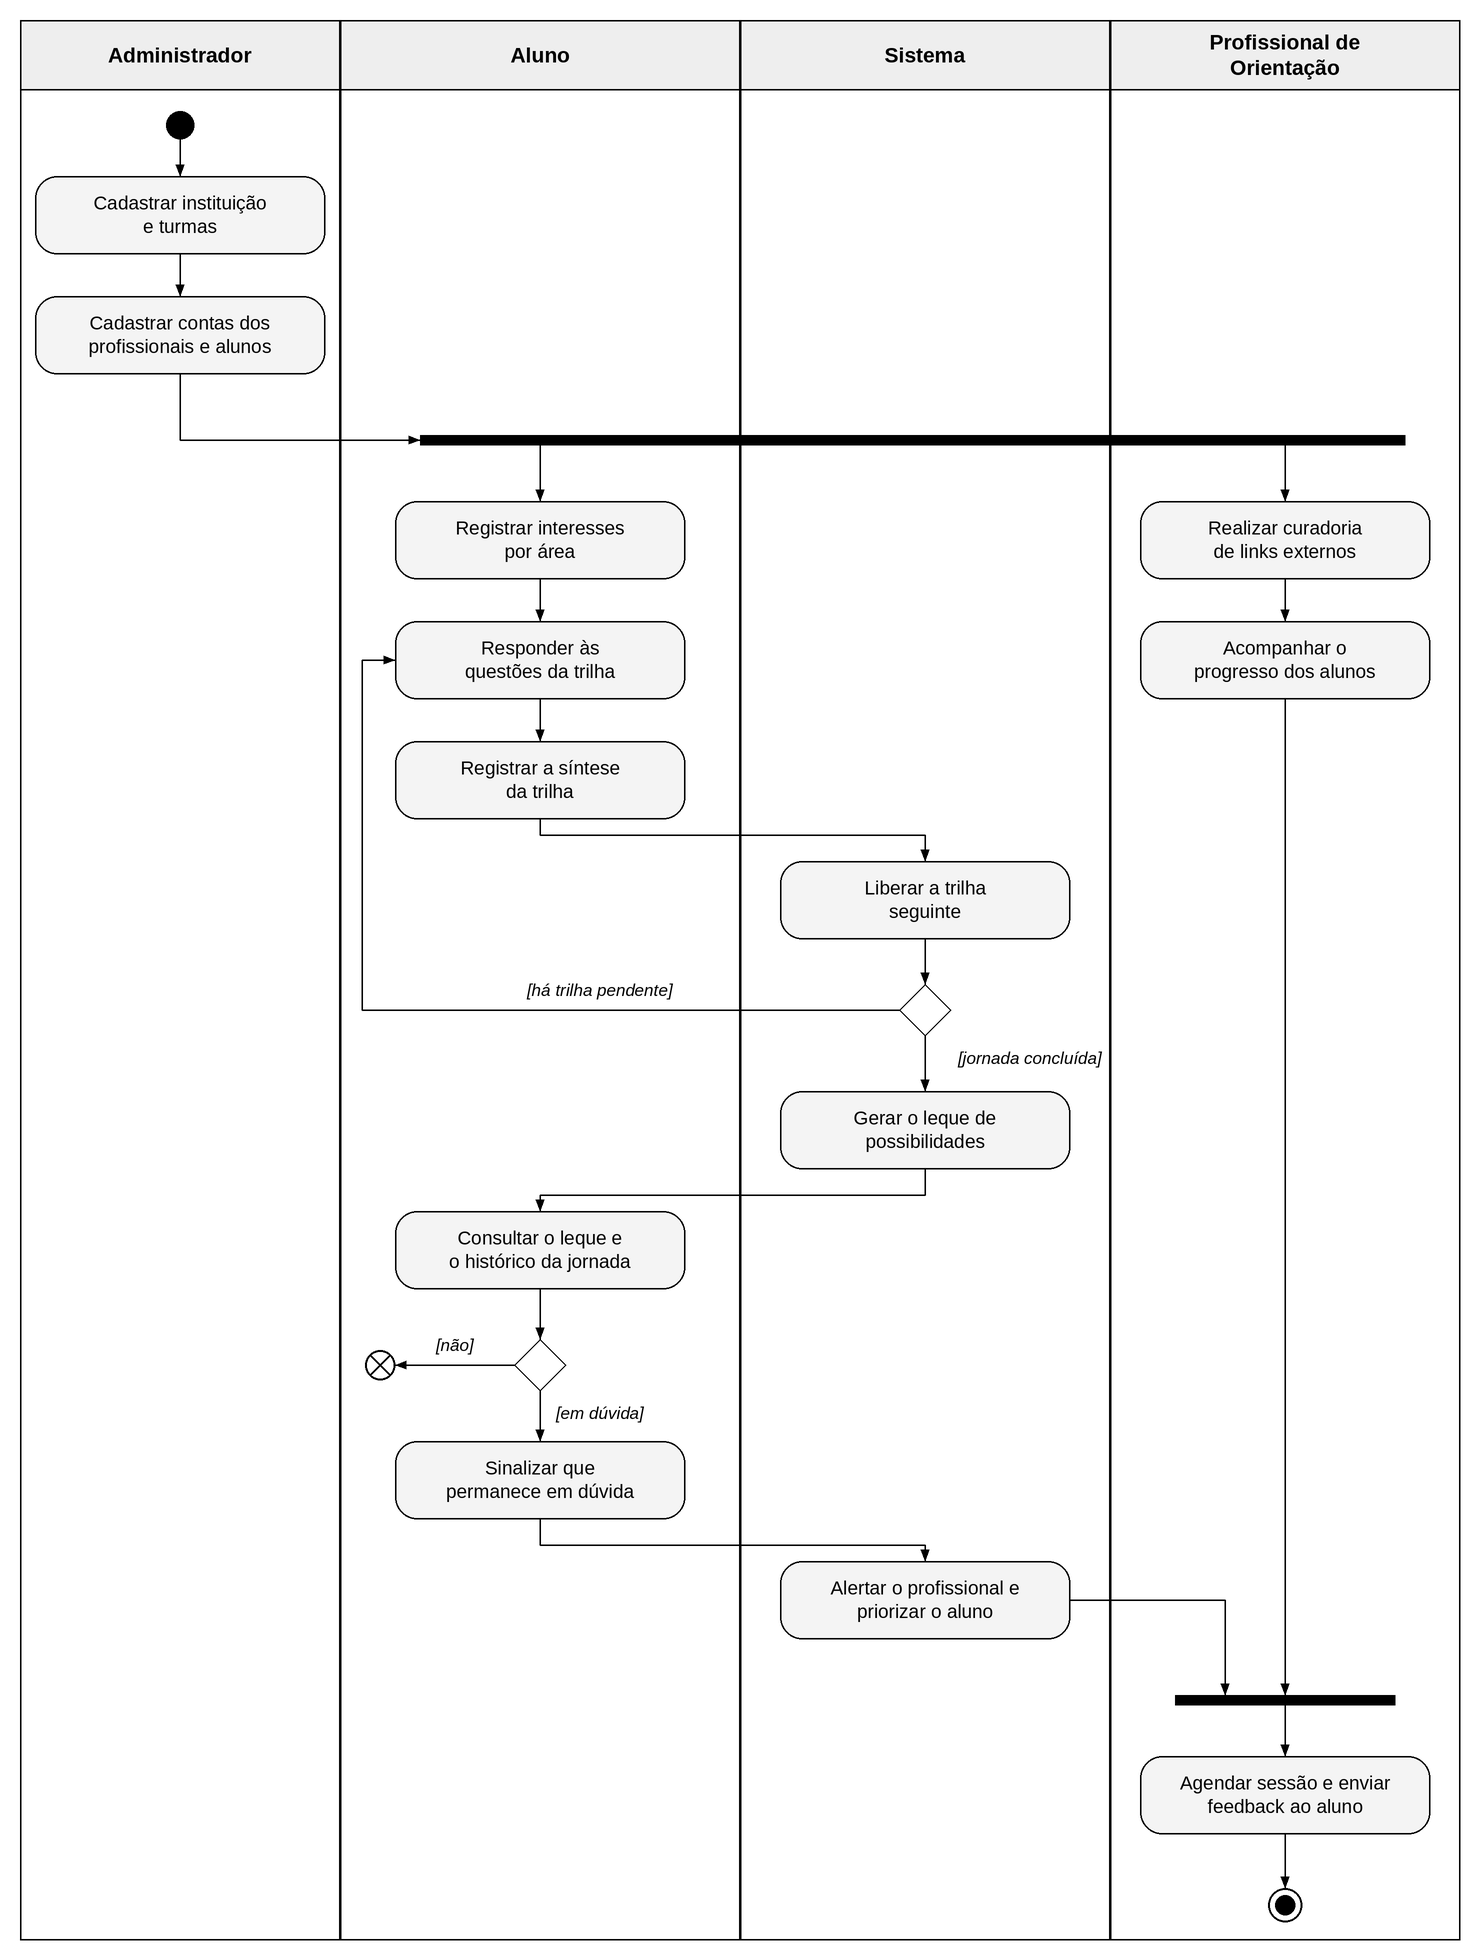
\includegraphics[width=0.92\textwidth]{img/fig-cap2-atividades.png}
    \legend{Fonte: Autoria própria (2026).}
\end{figure}
